% submit to https://sites.google.com/site/wpmvp2014/home
\documentclass[preprint]{sigplanconf}

% The following \documentclass options may be useful:

% preprint      Remove this option only once the paper is in final form.
% 10pt          To set in 10-point type instead of 9-point.
% 11pt          To set in 11-point type instead of 9-point.
% authoryear    To obtain author/year citation style instead of numeric.

\usepackage{amsmath}
\usepackage{listings}
\usepackage{hyperref}

\lstset{captionpos=b, float}

\usepackage{tikz}
\usetikzlibrary{positioning}
\usetikzlibrary{shadows}
\usetikzlibrary{arrows}
\usetikzlibrary{shapes}



\begin{document}

\special{papersize=8.5in,11in}
\setlength{\pdfpageheight}{\paperheight}
\setlength{\pdfpagewidth}{\paperwidth}

%\conferenceinfo{CONF 'yy}{Month d--d, 20yy, City, ST, Country} 
%\copyrightyear{20yy} 
%\copyrightdata{978-1-nnnn-nnnn-n/yy/mm} 
%\doi{nnnnnnn.nnnnnnn}

\title{Vectorizing Python Constructs Using Pythran and Boost SIMD}

\authorinfo{Serge Guelton}
           {QuarksLab, T{\'e}l{\'e}com Bretagne}
           {sguelton@quarkslab.com}
\authorinfo{Jo{\"e}l Falcou}
           {MetaScale}
           {joel.falcou@metascale.org}
\authorinfo{Pierrick Brunet}
           {INRIA/MOAIS}
           {pierrick.brunet@inria.fr}

\maketitle

\begin{abstract}

    The Python language is highly dynamic, most notably due to late binding. As
    a consequence, program run using Python typically run an order of magnitude
    slower than their C counterpart. It is also a high level languages whose
    semantic can be made more static without much change from a user point of
    view in the case of mathematical applications. In that case, the language
    provides several vectorization opportunities that are studied in this
    paper, and evaluated in the context of Pythran, an ahead-of-time compiler
    that turns Python module into C++ meta-programs.

\end{abstract}

%\category{CR-number}{subcategory}{third-level}

% general terms are not compulsory anymore, 
% you may leave them out
%\terms
%term1, term2

\keywords
Vectorization, Meta-Programming, Python, C++


%%
%%
\section{Python, Unboxing and Pythran}

The Python language has grown in audience for the past ten years, even reaching
the world of scientific computations thanks to the \texttt{numpy} module, a
%% what about the scipy module? It is not really used?
module that provides a MATLAB-like API. As a consequence, more and more code is
being written either in pure Python, generally to prototype an application, or
as a Python and native code mix when performance matters. However, Python
trades performance for dynamicity and does not particularly shines in terms of
performance.

For instance, the natural solution to Project Euler sixth problem ``Find the
difference between the sum of the squares of the first one hundred natural
numbers and the square of the sum`` can be coded as in
Listing~\ref{lst:euler06-py} in Python and as in Listing~\ref{lst:euler06-c} in
C. A comparison of the performance of the Python function and the C function
called through the \texttt{ctypes} module shows that the C version runs more
than $\times250$ faster than the Python version. Enabling compiler
auto-vectorization makes the C version $\times400$ faster than the Python
version.~\footnote{To perform more reliable time measurements, \texttt{n} has
    been increased to 100001 instead of 101. The script used to perform the
    measures as well as all other experimental data are available at
\url{https://github.com/serge-sans-paille/pythran/tree/wpmvp14/doc/papers/wpmvp14/experiments}.}

There are two main reason for the poor performance of Python:

\begin{description}

    \item[dynamic binding] each variable access is made through a dictionnary
        look-up to bind variable names to variable instances~;

    \item[boxing] each variable value is encapsulated into a heap-allocated
        generic object ---the \texttt{PyObject}--- which implies extra
        indirections for each operation.

\end{description}

In that context, it does not make sense to speak about vectorization: the
nature of an operation is unknown to the interpreter until its execution, and
data are not contiguous in memory.

\lstinputlisting[language=python, label={lst:euler06-py}, caption={Solution to the Project Euler Sixth Problem in Python}]{experiments/euler06.py}

\lstinputlisting[language=c, label={lst:euler06-c}, caption={Solution to the Project Euler Sixth Problem in C}]{experiments/euler06.c}

Several approaches have been proposed to solve these issues: using native
modules, relying on Ahead-Of-Time (AOT) or Just-In-Time (JIT) compilation.

A native module is a shared library whose interface make it callable from the
Python interpreter using the regular \texttt{import} mechanism. It makes it
possible to call native code from Python in a transparent way. Typically
%% It may be others languages, isn't it?
Python object are unboxed when transferred from Python to C, where efficient
computations can happen. Then the result is boxed when getting back to the
Python world. In between, vectorization can happen. This is the approach taken
by the \texttt{numpy} module: a native type, the \texttt{ndarray} contains
contiguous unboxed elements, and provides a great deal of high-level functions
to manipulate them. All the computation-intensive part is done in pure C.
Vectorization can eventually happen at this level, for instance when performing
a point-to-point operation like the sum of two arrays. However the granularity
of the operations limits the ratio of \texttt{load}/\texttt{store} versus operation. For
instance, if \texttt{a}, \texttt{b} and \texttt{c} are 1-D arrays, the sum
\texttt{a + b + c} is computed using two loops and an intermediate array.
% It means there are 4 load / stores and only two loops of addition.

AOT compilation uses type inference or type annotation to statically compute
the type of all (like in Shedskin, Parakeet) or part of (like in Cython or
Numba) variables, effectively unboxing them to speed-up computations. Using JIT
compilation, type information is available at runtime and the unboxing decision
is based on profitability, e.g.\ according to a trace analysis. This is the
approach of the PyPy project. In both cases, generation of vector instruction
is possible, but none of the cited project use it. Indeed automatic
vectorization is a complex topic, and as stated in~\cite{maleki2011}, many cases
are not yet correctly supported even for mainstream compilers.

Pythran is also an AOT compiler, which holds the unique property of turning
Python modules into C++ \emph{meta-programs}. It does not need type annotations
and keeps the polymorphism of original functions, respecting Python's duck
typing. Its compilation workflow is described in Figure~\ref{fig:pythran-compiler}.
Like others AOT compilers, it unboxes all variables for better performance, and
performs a wide variety of optimizations such as lazy evaluation, constant
folding, expression fusion etc. It supports core \texttt{numpy} constructs and
most Python constructs to the notable exception of user classes. Constructs
such as \texttt{eval}, are not supported.


\begin{figure}

\centering
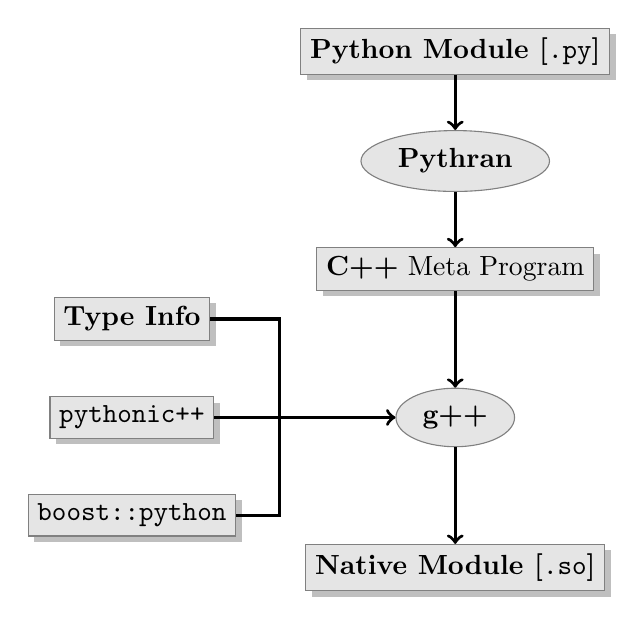
\begin{tikzpicture}[
file/.style={draw=black!50,fill=black!10,rectangle, drop shadow, align=center,
node distance=0.7cm},
    tool/.style={draw=black!50,fill=black!10,ellipse, align=center, node
    distance=0.7cm}]
    \node[file] (python) {\textbf{Python Module [\texttt{.py}]}};
    \node[tool] (pythran) [below=of python] {\textbf{Pythran}};
    \node[file] (meta-cxx) [below=of pythran] {\textbf{C++} Meta Program};
    \node[tool] (gxx) [yshift=-1.5em, below=of meta-cxx] {\textbf{g++}};
    \node (empty) [xshift=-1em, left=of gxx] {};
    \node[file] (pythonic) [left=of empty] {\textbf{\texttt{pythonic++}}};
    \node[file] (annotation)     [above=of pythonic] {\textbf{Type Info}};
    \node[file] (boost) [below=of pythonic] {\textbf{\texttt{boost::python}}};
    \node[file] (so) [yshift=-1.5em, below=of gxx] {\textbf{Native Module
    [\texttt{.so}]}};

\draw[very thick, ->] (python) -- (pythran);
\draw[very thick] (annotation) -| (empty.center);
\draw[very thick, ->] (pythran) -- (meta-cxx);
\draw[very thick, ->] (meta-cxx) -- (gxx);
\draw[very thick] (boost) -| (empty.center);
\draw[very thick, ->] (pythonic) -- (gxx);
\draw[very thick, ->] (gxx) -- (so);
\end{tikzpicture}

\caption{Pythran compiler workflow.}
\label{fig:pythran-compiler}
\end{figure}


This paper introduces vectorization of Python programs based on the idea that
many Python constructs already exhibit good vectorization opportunities. The
goal of the paper switches from automatic vectorization to vectorization of
high-level Python intrisics, as described in Section~\ref{sec:python-semantic}.
One of the difficulties of vectorizing Python functions is linked to function
polymorphism. Vectorization in the context of C++ meta-programs is examined in
Section~\ref{sec:meta-vectorization}. The approach is validated using the
Pythran compiler on several micro-applications from signal processing, physics
and mathematics presented in Section~\ref{sec:benchs}.

%%
%%
\section{Vectorization of a Meta-Program}
\label{sec:meta-vectorization}

\subsection{Boost SIMD}

\subsection{\texttt{Load}/\texttt{Store} Protocol}


%%
%%
\section{Using Python Semantic for Vectorization}
\label{sec:python-semantic}

Automatic vectorization generally relies on explicit loop-level vectorization, as
extensively described in~\cite{bik04}, or on block-level vectorization, also
called Superword Level Parallelism (SLP) as introduced in~\cite{larsen00}.
Modern compilers for C/C++/FORTRAN generally implement a mixture of both.

A high-level language such as Python exhibit another level of vectorization
opportunity in implict loop. Implicit loops can be found in many places, but
this paper focuses on \emph{list comprehension} and \emph{generator
expression}, \emph{map} or \emph{sum} intrinsics and \emph{array operations}
through the \texttt{numpy} module.

\subsection{Intrinsics}

\subsubsection{\texttt{sum}}
% only sum as texttt in a title is not really beautiful

The \texttt{sum} intrinsic is a typical case of potential vectorization of an
implict loop. Its prototype is: \texttt{sum(sequence[, start]) $\rightarrow$
value} and its behavior is equivalent to the Python code in
Listing~\ref{lst:sum-py}. Depending on the type of \texttt{sequence}, and also
wether one needs to strictly conforms to the IEEE Standard for Floating-Point
Arithmetic (IEEE 754).
% I don't understand what this last sentence is doing here :-s

\begin{lstlisting}[language=python, label={lst:sum-py}, caption={Pseudo code of the \texttt{sum} intrinsic.}]
def sum(sequence, value=0):
  for e in sequence:
    value += e
  return value
\end{lstlisting}


Appart from standard compliancy, to be able to efficiently vectorize this code in C++, one must check that:

\begin{enumerate}
    \item\label{enu:same-types} All element of \texttt{sequence} have the same types;
    \item\label{enu:scalar-types} \texttt{sequence} contains scalar types;
    \item\label{enu:contiguous} \texttt{sequence} contains contiguous elements;
    \item\label{enu:random-access} \texttt{sequence} provides a random access iterator. In particular one can computes its size in $\mathcal{O}(1)$.
\end{enumerate}

Condition~\ref{enu:same-types} is a prerequiste for static typing and efficient
unboxing. For instance, any code that does not match it will fail to compile
using Pythran or Shed-Skin. It is also satisified for the \texttt{ndarray}
container as they wraps unboxed arrays. Condition~\ref{enu:scalar-types} can be
checked at compile time. Python supports two native scalar types candidates for
vectorization: \texttt{int} (64 bits integer) and \texttt{float}
(double-precision floating point numbers). The \texttt{numpy} model add supports for a
wide range of signed and unsigned integers as well as single, double or
quadruple precision float. Depending on the target architecture, only some of
them can fit into vector registers. Finally condition~\ref{enu:contiguous} also
is a static property of a container. It is verified for C++ alternative to
Python's \texttt{list}, \texttt{str} and \texttt{ndarrays}, but generally not
for \texttt{set} or \texttt{dict}. Condition \ref{enu:random-access} is not
matched by \emph{generator}s, the Python incarnation of co-routines.

%we know a work have to be done about random acces but you speak about something else now ...
%It is disturbing and we don't really know why you speak about this new topic.

As function have to be generic but some containers do not match requierement
properties, it is possible to select a vectorized
implementation of fallback to a generic one using Substitution Failure
Is Not An Error (SFINAE).

A possible C++ meta-implementation of \texttt{sum} in that context is presented
in listing~\ref{lst:sum-cxx}. It makes use of the parametric vector register
introduced by Boost.SIMD and presented in Section~\ref{sec:meta-vectorization}.
There is nothing new in the vectorization scheme itself. However, the
possibility to write a meta-function that provides a vectorized implementation
of the \texttt{sum} intrinsic makes it possible to efficiently turn a Python
call into a C++ call.

\begin{lstlisting}[language=c++, label={lst:sum-cxx}, caption={Meta-implementation of the \texttt{sum} intrinsic in C++11.}]
template<class T, class V=long>
typename std::enable_if<is_vectorizable<T>::value,
                        typename T::value_type
                       >::type
sum(T const& sequence, V value=0L)
{
  // E is the type of an element of T
  typedef typename T::value_type E;
  // vE is a vector type of vsize elements of type E
  typedef typename simd::native<E,
    BOOST_SIMD_DEFAULT_EXTENSION> vE;
  static const size_t vsize =
    simd::meta::cardinal_of<vE>::value;

  // vector_value is for the parallel reduction
  vE vector_value = simd::splat<vE>(E());
  const size_t n = sequence.size();
  const size_t bound = n / vsize * vsize;
  for(size_t i = 0; i < bound; i+= vsize)
    vp += sequence.load(i);
  // inner sum of the vector
  value += boost::simd::sum(vp);

  // handle the tail
  for(size_t i = bound; i < n; ++i)
    value += sequence.at(i);
  return value;
}
\end{lstlisting}

\subsubsection{\texttt{map}}

The \texttt{map} intrinsic simply creates a new \texttt{list} and fills it by
repeatedly applying a function to the items of its argument sequence(s). Its
prototype is: \texttt{map(function, sequence[, sequence, \dots]) $\rightarrow$
list}. Again, this is a typical case of vectorizable implicit loops, providing
some conditions are met:

\begin{enumerate}

    \item[\label{enu:pure}] \texttt{function} must be vectorizable;
    \item[\label{enu:sequence}] all \texttt{sequence}s verify the same constraints as stated for the \texttt{sum} intrinsic.

\end{enumerate}

Deciding if a given function is vectorizable can be approximated through a
composition rules. First, some functions are known to be vectorizable. This is
generally the case for the addition, subtraction etc. Depending on the target
vector instruction set, some operations may or may not be available as vector
instructions, e.g.\ trigonometric functions, but they can be provided as
composite instructions. Some are just not available, as quadruple precision
float addition. Starting from this set of vectorizable function, one can use
the \texttt{;} as a closure binary relation to compute a subset of all
vectorizable functions. Said otherwise, any sequence of operation that only
involve vector operations is a vector operation and a function whose body is a
sequence of vector operation or vectorizable functions is a vectorizable
function itself.

The preceding statement is only valid if the function's body only references
vector functions and formal parameters, as the function must be valid for both
scalar types and vector types. Note that this perfectly matches the translation
of polymorphic Python functions into C++ meta-functions, as detailed in
Listings~\ref{lst:square-python} and~\ref{lst:square-cxx}. The core idea is that
the \texttt{square} function can be called indifferently on floating point
values or on vector of floating point values. Through (automatic) template
instantiation, the C++ compiler generates the actual scalar and vector version
from the same meta-function. As Pythran always translates Python's polymorphic
function in that form, writing a vector version of the \texttt{map} intrinsic is
slightly more difficult than for the \texttt{sum} intrinsic due to its variadic
number of arguments, but it also relies on the \texttt{load}/\texttt{store}
protocol and SFINAE to select it.

\begin{lstlisting}[language=python, label={lst:square-python}, caption={Python implementation of the square function.}]
def square(x):
  return x * x
\end{lstlisting}

\begin{lstlisting}[language=c++, label={lst:square-cxx}, caption={C++ meta-implementation of the square function.}]
struct square {
    template<class T>
    auto operator()(T const& x)
    -> decltype(x * x)
    {
      return x * x;
    }
};
\end{lstlisting}

\subsection{List Comprehension}

Python provides \emph{list comprehension} as a way to create \texttt{list} from
any iterable. For instance \texttt{[abs(x) for x in l]} creates a new
\texttt{list} that holds the absolute value of each element of \texttt{l}. A
filter can be set up as in  \texttt{[abs(x) for x in l if x \% 3]}, where only
the elements non multiple of 3 are taken into account. Let us call
\emph{comprehesion rule} the expression on the left of the
\texttt{for}.

List comprehension can be translated into a combination of \texttt{map} and
(optionnaly) \texttt{filter}, by transformation of the comprehension rule into
a lambda function. For instance the previous example can be re-written as
\texttt{map(abs, filter(lambda x: x\% 3, l))}. Once in this form, the same
    vectorization opportunities as in the previous section arise.

Generator expression is somehow similar to list comprehension, to the notable
exception that the value returned is an \emph{iterator adaptator} on the
container argument. In the context of vectorization, a generator expression
supports the vector protocol if the associated container also supports it. In
that case the  \emph{iterator adaptator} implements the vector protocol by
applying the comprehension rule to each vector element from this container, in a
streaming fashion.

Python also provide same features for set and dictionnary.

Set comprehension can also be rewritten in the form of
generator expression using the eponym function: \texttt{\{ x + 3 for x in l\}}
is equivalent to \texttt{set(x + 3 for x in l)}.

Dictionnary comprehension and multi-level comprehension (i.e.\ containing
multiple \texttt{for} clauses) are not considered in this preliminary work.

\subsection{The Numpy Module}

The \texttt{numpy} module played a major role in the adoption of Python by the
scientific community. In a nutshell, this is a thin Python wrapper above a raw
array that provides an array language embeded into Python. An example of
\texttt{numpy} code is show on Listing~\ref{lst:numpy-code}.

\begin{lstlisting}[language=python, label={lst:numpy-code}, caption={Sample \texttt{numpy} code.}]
import numpy as np
def rosen(x):
  return np.sum(100*(x[1:] - x[:-1] ** 2) ** 2
                + (1 - x[:-1]) ** 2)
\end{lstlisting}

Common features of array language include indexing, slicing, point-to-point
operation etc. The latter is traditionnaly a good source of vectorization.
However, because of the module layer, \texttt{numpy} always create a new array
to hold intermediate result. For instance in the expression \texttt{(1 -
x[:-1]) ** 2)} two array are created ---slicing does not create an array but a
view. The implied extra cost would hide the benefits of vectorization.

The typical way to solve this issue in C++ is to use \emph{expression
templates}, a technique described in~\cite{} that uses the C++ type system to
perform lazy evaluation of an expression. However, this approach is limited to
a single expression. Listing~\ref{lst:numpy-code-fs} illustrates the situation:
expression templates would not prevent the creation of temporary arrays
\texttt{t0} and \texttt{t1}. Fortunately, it is possible to apply \emph{forward
substitution} to fallback to the expression from Listing~\ref{lst:numpy-code}
and avoid the creattion of any temporary.

\begin{lstlisting}[language=python, label={lst:numpy-code-fs}, caption={Sample \texttt{numpy} code requiring forward subsitution.}]
import numpy as np
def rosen(x):
  t0 = 100*(x[1:] - x[:-1] ** 2) ** 2
  t1 = (1 - x[:-1]) ** 2
  return np.sum(t0 + t1)
\end{lstlisting}

It is possible to hook in the expression template to add vectorization support.
Indeed the expression from Listing~\ref{lst:numpy-code} hides a single vector
loop, that can be explicitly vectorized using Bosst.SIMD in a similar manner as
the \texttt{map} and \texttt{sum} intrinsics.

One potential drawback of the approach would be the generation of multiple load
from the same location, as in \texttt{1. / a + a}, where \texttt{a} is loaded
twice on each loop iteration. Fortunately, the backend C++ compiler is capable
of detecting the redundant load and perform \emph{redundant load store
elimination}, effectively issuing a single load.

%%
%%
\section{Validation of the Approach using the Pythran Compiler}
\label{sec:benchs}

\acks

Acknowledgments, if needed.

% We recommend abbrvnat bibliography style.
\cite{*}

\bibliographystyle{abbrvnat}
\bibliography{biblio}


\end{document}
